%LaTeX Document
\documentclass[a4paper,twoside,12pt]{article}
\usepackage{xltxtra}
\usepackage{url}
\setromanfont[Mapping=tex-text]{TeX Gyre Pagella}
\setsansfont[Mapping=tex-text]{DejaVu Sans}
\setmonofont[
  Mapping=tex-text,
%  Scale=0.85,
  AutoFakeSlant,
  BoldItalicFeatures={FakeSlant}]{Inconsolata}
%\newfontfamily{\A}[Scale=0.85]{DejaVu Sans} % TODO find a free Arial/Helvetica equivalent
%\newfontfamily{\J}[Scale=0.85]{Hiragino Kaku Gothic Pro}
%\newfontfamily{\P}[Scale=0.85]{Palatino}
%\usepackage{soul} % Pour barrer

%%%%%%%%%%%%%%%%%%%%%%%%%%%%%%%%
%%         BEGIN FIXME         %
%%%%%%%%%%%%%%%%%%%%%%%%%%%%%%%%
\def\plongday{Samedi}
\def\pday{14}
\def\pmonth{mai}
\def\pyear{2016}

\def\ptitle{Guide des bonnes pratiques pour la construction et la
maintenance de tuyaux extracteurs cosmiques à vacuité} %% Subject's main title
\def\psubtitle{CONFIDENTIEL\\Informations destinées au personnel détenant la
certification RS232RJ45-B/α} %% Subject's sub title

\def\plogo{prologin2016.pdf} %% Logo
\def\psubjectpicture{image.png} %% Picture to be displayed
%% on its own page

%%%%%%%%%%%%%%%%%%%%%%%%%%%%%%%%
%%         END FIXME           %
%%%%%%%%%%%%%%%%%%%%%%%%%%%%%%%%


%%%%%%%%%%%%%%%%%%%%%%%%%%%%%%%%%%%%%%%%%%%%%%%%%%%%%%%%
%%              DO NOT EDIT PAST THIS LINE            %%
%%%%%%%%%%%%%%%%%%%%%%%%%%%%%%%%%%%%%%%%%%%%%%%%%%%%%%%%











%\documentclass[a4paper,twoside,12pt]{book}

\usepackage[french]{babel} % TODO switch to polyglossia?
\usepackage{geometry}
\usepackage{multicol}
\usepackage{fancyhdr}
\usepackage{listings}
\usepackage{array}
\usepackage{color}

\def\pdate{\plongday{} \pday{} \pmonth{} \pyear{}}

\definecolor{colIdentifier}{gray}{0}
\definecolor{colKeys}{rgb}{0,0,0.6}
\lstset{
    extendedchars=false,
    showstringspaces=false,
    escapeinside=@@,
%    keywordstyle=\color{blue},
%    commentstyle=\color[rgb]{0.133,0.545,0.133},
    columns=flexible,
    language=C++,
    tabsize=2,
    basicstyle=\ttfamily\NoAutoSpacing
%    numbers=left,
%    frame=lines
}
\lstnewenvironment{lst-c++}{%
\lstset{%
language=C++
}}{}


%\renewcommand\ttdefault{cmtt}

\newcommand{\functitle}[1]{%
\vspace{0.5cm}
$\bullet$ \underline{\textbf{#1}}
}

%\NoAutoSpaceBeforeFDP
\geometry{bindingoffset=5mm,hmarginratio=1:1,heightrounded,headheight=15pt}

\makeindex

\begin{document}
\pagestyle{empty}
\sloppy

%\lhead[\textsl{Prologin 2009}]{\nouppercase \leftmark}
%\rhead[Sujet de la finale]{}
\lhead[\thepage]{\nouppercase \leftmark}
\rhead[\textsl{Prologin \pyear{}} --- Sujet de la finale]{\thepage}
\cfoot{}

% Couverture =========================================================
\begin{titlepage}
\begin{center}
~\includegraphics[width=\linewidth]{\plogo}\\
\vspace{5cm}
\Huge
\textbf{\ptitle{}}

\vspace{1cm}

\Large
\textbf{\psubtitle{}}

\vspace{2cm}

\normalsize
\textnormal Sujet de la finale du Concours National d'Informatique\\
\pdate\\
\end{center}
\end{titlepage}

\small

% Sommaire ===========================================================
\cleardoublepage
\tableofcontents

\normalsize

% Corps ==============================================================
%\cleardoublepage
\setcounter{page}{1}
\pagestyle{fancy}
\parskip=6pt plus 3pt

\newpage

\vspace{4cm}

\begin{center}\includegraphics[height=14cm]{\psubjectpicture}\end{center}

\newcommand{\provogon}{ProVogon™}

\vspace{-1cm}

\noindent\emph{Ô blas bougriot glabouilleux\\
Tes micturations me touchent\\
Comme des flatouillis slictueux\\
Sur une blotte mouche\\
Grubeux, je t'implore\\
Car mes fontins s'empalindroment\ldots\\
Et surrénalement me sporent\\
De croiçantes épiquarômes.\\
Ou sinon\ldots nous t'échierons dans les gobinapes\\
Du fond de notre patafion\\
Tu verras si j'en suis pas cap!
}

\vspace{1cm}

\hspace{5cm} --- Poème Vogon

\newpage

\section{Introduction}

\vspace{1cm}

\textbf{Bienvenue à \provogon{}.}

Si vous lisez ces lignes, c'est que vous faites partie des rares individus de à
avoir passé nos entretiens (avec brio !), et faites enfin partie de notre
grande famille\footnote{Parlez de nous à vos amis, on recrute.}. Félicitations !

Prenez quelques minutes pour méditer sur votre exploit : si vous êtes parvenus
jusqu'ici, c'est que :

\begin{itemize}
    \item vous faites partie des 3 103 274 212 112 ayant postulé en remplissant
        les formulaires 1149, 1459 et 802.11 sur \texttt{RS-123 BETELGEU\~1} ;
    \item vous avez successivement passé l'épreuve du feu, l'épreuve de l'eau,
        l'épreuve du vent, l'épreuve de la chaussure qui fait un peu mal au
        gros orteil, la dictée à dos de cheval et le remplissage de formulaire
        peu clair, imprécis et légèrement embarrassant ;
    \item vous avez découvert la série d'indices qui vous menait à la planète
        SOL3, en prenant la première à gauche après Proxima ;
    \item vous avez trouvé le faux concours d'informatique qui nous servait de
        couverture pour dissimuler nos activités sur cette planète primitive ;
    \item vous avez prouvé que vous faisiez bien partie de nos meilleurs
        candidats en réussissant nos épreuves d'informatique\footnote{Bien
        entendu, ces épreuves étaient bien trop dures pour être résolues par de
        simples humains, il n'y a donc aucun risque que les autochtones soient
        parvenus jusqu'ici.}.
\end{itemize}

Nous vous remercions également d'avoir signé notre fausse autorisation de
diffusion d'image, dont vous avez bien sûr relevé la mention en
petites\footnote{7 nanomètres de largeur, au-dessus du minimum prévu par la
loi.} lignes retranscrite ci-dessous :

\emph{Je m'engage également à exercer au sein de la société \provogon{} les
fonctions d'ingénieur-architecte constructeur de niveau 4, à me conformer aux
dispositions conventionnelles en vigueur dans la société \provogon{} pour une
durée indéterminée comprenant une période d'engagement non-interruptible de
2455 années terrestres, en vertu du code du travail en vigueur dans le système
étatique du sous-groupe galactique Gamma.}

Nous imaginons très bien la joie que vous devez ressentir à l'idée de
collaborer avec notre entreprise. Ce petit guide qui vous a été remis a
plusieurs objectifs. Tout d'abord, vous présenter \provogon{}, ses différents
aspects, ses valeurs, ses engagements, et tous les avantages qu'elle vous
apportera dans votre parcours professionnel. Ensuite, vous détailler en quoi
consistera votre rôle et vos objectifs pour bien entamer votre carrière parmi
nous.

Bon courage !

\section{Présentation de \provogon{}}

\subsection{Notre activité}

Fondée il y a plusieurs millions d'années\footnote{\provogon{} Authentic,
depuis -273 283 102 (Appellation d'Origine Contrôlée).} par deux frères Vogons,
l'entreprise de construction \provogon{} a commencé son activité par de simples
terraformations de planètes recyclables.  La qualité des prestations de
\provogon{} lui a peu à peu permi de se faire connaître dans les hautes
sphères, ce qui lui a permis d'étendre son activité dans l'assemblage de
systèmes planétaires, la mise en orbite de satellite naturels, les spectacles
d'éclipse, la mise en place de soleils de plaisance ainsi que la destruction de
planètes qui gâchent un peu la vue.

Ainsi, après seulement quelques petits millions d'années d'existence, \provogon{}
est devenue l'entreprise de référence en construction spatiale, ce qui lui a
permis de s'attaquer à de nouveaux secteurs d'activités encore inexplorés,
comme l'arrachage chirurgical de branches de galaxies ou le dépannage et
tractation des vaisseaux coincés au delà de l'horizon des événements des trous
noirs de petite et moyenne taille.

\subsection{Notre modèle économique}

Pour faire simple, toutes les études de marché sont claires sur un point :
l'internalisation des externalités rencontrent certaines limites comme la
rationalité limité des agents ou l'incohérence inter temporelle, c'est pourquoi
la fiscalité patrimoniale des institutions politico-internationales légales
s'impose d'elle même par la construction emphasique des inégalités sur le
terrain, à la fois covariantes et contravariantes. Nous tirons ainsi notre
stratégie principalement de la taxation quadratique des agents commerciaux
indépendants, notamment dans le cadre de biens substituables par effet de
concurrence et de découragement. On a ainsi affaire à un problème de TGO
(Théorie Générale des Organisations), pour avoir la vogolexicomatisation des
lois du marché propre par sa nucléarité, vous l'aurez compris.

\subsection{Nos valeurs}

\subsubsection{Productivité}

\emph{« Pour assurer le retour à une croissance à deux chiffres, le dirigisme
paternaliste de naguère a laissé place à l'horizontalité d'une gestion
collaborative encadrée par des chefs d'équipe qualifiés. Plus un seul
collaborateur n'aura à craindre le flétrissement de l'immobilisme. La
flexibilité naturelle de l'homme moderne ne sera plus contrariée par aucune
entrave. Motivés par leur désir de développement personnel et leur esprit
d'entreprise, les équipes rejoignent chaque matin leur poste de travail, leur
cœur vaillant battant au rythme des propositions des managers dynamiques. »}

\vspace{0.3cm}
\hspace{3cm} --- Maciste contre le Capital

À \provogon{}, notre priorité absolue est la productivité de nos employés. Nous
croyons au sacrifice de soi pour s'assurer une brillante carrière. Nous ne
pouvons donc pas tolérer que nos employés perdent de précieuses minutes
d'inattention, au risque de baisser significativement lors de leurs revues de
performance quotidiennes.

Rassurez-vous : nous avons tout prévu pour que vous n'ayez pas à vous poser de
questions. Nous installerons dès que possible un appareil qui vous permettra
de rester concentré et attentif en toutes circonstances, en vous envoyant
régulièrement des décharges électriques afin que chacun de vos neurones reste
dédié à la tâche qui vous est confiée. Tout est plus simple chez \provogon{} !

\subsubsection{Avantages des associés}

En tant qu'associé de \provogon{}, les avantages dont vous disposez sont nombreux :

\begin{itemize}
    \item plusieurs dizaines de minutes de repos par jour\footnote{Pendant
        lesquelles vous serez d'astreinte, bien sûr.} ;
    \item 5 semaines de congés payés par siècle ;
    \item des primes importantes en cas d'accident du
        travail\footnote{Rassurez-vous, ceux-ci sont assez réguliers pour
        que ces compensations soient importantes !} ;
    \item et bien d'autres\footnote{Vous les découvrirez bien assez tôt.} !
\end{itemize}

\subsubsection{Engagements qualité}

\provogon{} attache une importance toute particulière à la qualité de ses
prestations. Nous vous demandons pour cela de suivre à la lettre ces quelques
consignes simples.

Chaque modification, avant d'être implémentée, doit être minutieusement passée
en revue au minimum par les dix-sept premiers niveaux de hiérarchie
immédiatement supérieurs à l'employé à l'origine du changement.  Lors de ce
procédé, chaque personne de la chaine doit remplir le formulaire Q747
\textbf{bleu} pour les personnes de rang \textbf{pair} en partant du haut, et
le formulaire Q747 \textbf{vert citron} pour les personnes de rang
\textbf{impair}.

Une fois que l'autorisation de principe est ainsi obtenue, le chargé
d'implémentation (qui sera détenteur d'au moins trois demi-douzaines de
certifications relatives au domaine concerné) devra écrire un rapport
fonctionnel détaillé sur chaque ligne de code, qui seront ensuite relus par des
personnes choisies au hasard dans l'entreprise.

La validation du changement se fera à la suite d'une soutenance avec des slides
présentant ses avantages et inconvénients, ainsi que des tests unitaires, des
tests d'intégration, des tests de performance, des fiches de test, le tout
présenté sur une centaine de graphiques très clairs.

L'implémentation relue, validée, certifiée, authentifiée et prouvée pourra
ainsi être intégrée au processus d'intégration qui a lieu tous les 18 mois.

\subsection{Votre mission}

Toute notre activité requiert une énergie importante, et vous avez été recrutés
pour faire partie des effectifs ayant pour mission la tâche de la plus haute
importance : collecter l'énergie nécessaire au bon déroulement de nos travaux.

Notre collecte d'énergie est entièrement non-polluante, en utilisant des
énergies renouvelables qui ne dégagent absolument pas de dioxyde de carbone :
nous \textbf{aspirons des étoiles} (des pulsars, plus précisément) à l'aide de
\textbf{tuyaux géants}, afin de capturer le plasma qui en ressort. Vous serez
tout simplement chargés de diriger ces opérations de collecte.

Évidemment, comme dans toute entreprise qui se respecte, vous ne pourrez pas
travailler d'égal à égal, c'est pourquoi nous devons vous hiérarchiser aussi
vite que possible.

Nous allons procéder de la façon suivante : nous allons vous placer dans une
simulation d'une situation réelle de sites de récolte de plasma, et vous vous
affronterez les uns contre les autres (à raison de deux personnes par partie).

La seule chose qui nous intéresse est la quantité de plasma que vous serez
capables de collecter, c'est pourquoi vous serez uniquement évalués sur cette
mesure.

Les sites sur lesquels vous travaillerez prennent la forme de carrés en 2
dimensions. Ceux-ci sont particulièrement singuliers car ils présentent une
forte concentration en pulsars qui émettent séquentiellement du plasma autour
d'eux. Le plasma émis apporte l'énergie dont nous avons besoin. Cependant, il
est hautement instable et ne peut se maintenir dans l'espace de façon autonome.
Le seul moyen de le récolter est de le maintenir enfermé dans des tuyaux
jusqu'à une base de collection.

Des bases sont disponibles sur la bordure de ces sites et permettent de
récupérer l'énergie du plasma. Sur un site donné, chacun des deux opposants
disposera de la moitié des bases, l'un occupera les bases au Nord et au Sud
tandis que l'autre disposera de celles à l'Est et à l'Ouest.

Pour permettre le transport du plasma des pulsars vers vos bases vous
disposerez d'une quantité illimitée\footnote{Illimitée ! Quelles conditions de
travail formidables.} de tuyaux.

Chaque base possède une puissance d'aspiration électro-magnétique permettant de
piéger le plasma et de l'attirer vers elle. Cette aspiration se propage le long
des tuyaux avec une atténuation constante.  Lorsqu'un plasma est relié à une
base par le réseau de tuyaux, il est soumis à cette attraction. Comme il peut
être attiré vers plusieurs directions à la fois, il se déplace à chaque instant
dans la direction où l'attraction est la plus forte, et il se divise en parts
uniformes s'il fait face à plusieurs forces d'attraction identiques provenant
de directions différentes.

Chaque base est initialement chargée d'une unité de puissance d'aspiration,
vous aurez la possibilité d'en déplacer des unités d'une case de base vers une
autre, en faisant attention de ne pas dépasser une certaine limite qui pourrait
déclencher une surcharge d'énergie.

Pour corser la partie (et imiter de façon réaliste la fourberie de nos
concurrents), il est également possible de détruire les tuyaux présents sur le
site, quel que soit le joueur qui l'ait construit. Cependant, une fois détruit,
un tuyau laisse des débris empêchant de construire par dessus sans déblayer le
lieu au préalable.

En guise de défense, il est également possible d'améliorer les tuyaux
existants. Un super tuyau sera plus coûteux à détruire et tout plasma qui passe
dedans verra sa vitesse doubler temporairement (c'est à dire qu'il se déplacera
de deux cases à la fois à chaque tour).

Vous serez évalués sur un temps fixé à l'issue duquel un vainqueur sera
désigné. Initialement le site est vide et ne contient que les pulsars, certains
d'entre eux pourront cesser d'émettre au cours de la partie, car ils disposent
d'une quantité de plasma finie. À vous de jouer pour en récolter un maximum !


\section{Cahier des charges}\label{cahier-des-charges}

\subsection{Site}\label{site}

Chaque site consiste en une grille carrée de \texttt{TAILLE\_TERRAIN}
cases de côté. Au centre de chaque bord se trouve une rangée de bases de
\texttt{LONGUEUR\_BASE} cases, encadrée de zones interdites de chaque
côté. Le reste de la région est constitué de pulsars et de cases vides.

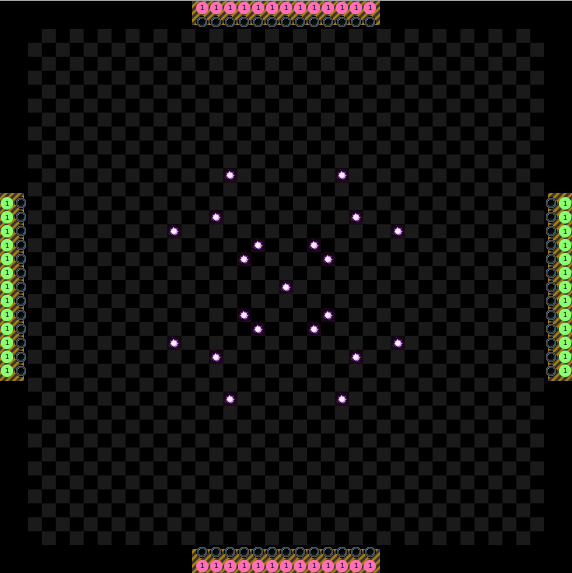
\includegraphics{../subject/slides/pictures/map.png}

\subsubsection{Base}\label{base}

Les bases se trouvant sur deux bords opposés appartiennent au même
joueur. Chaque case possède initialement une unité de puissance
d'aspiration, qui pourra être assignée à d'autres cases en cours de jeu,
dans la limite de \texttt{LIMITE\_ASPIRATION} unités par case.


\includegraphics{asset/base.png}

{Trois cases de base (au sud) de puissance d'aspiration 1, 2 et 1.}

\subsubsection{Zone interdite}\label{zone-interdite}

Ce sont les cases du bord des sites qui ne sont pas des cases de base,
il n'est pas possible de construire par dessus.


\includegraphics{asset/interdit.png}

{La zone interdite, en rouge, de part et d'autre d'une base (au sud) de taille 3 sur un site de côté 9.}

\subsubsection{Vide}\label{vide}

Ce sont des cases qui ne contiennent rien, la seule action possible est
de construire par dessus.


\includegraphics{asset/vide.png}

{Du vide entre deux tuyaux.}

\subsubsection{Pulsar}\label{pulsar}

Un pulsar a une position fixe, et possède des caractéristiques qui lui
sont propres :

\begin{itemize}
\tightlist
\item
  une période de pulsation \emph{T};
\item
  une puissance de pulsation \emph{P};
\item
  un nombre de pulsations restantes \emph{R}.
\end{itemize}


\includegraphics{asset/pulsar.png}

{Un pulsar.}

\subsubsection{Tuyau}\label{tuyau}

Le tuyau est un composant qui permet de transporter le plasma. Les
effets d'un tuyau (ou d'un Super-Tuyau™) ne dépendent pas du joueur qui
l'a construit.


\includegraphics{asset/tuyau.png}

{Trois tuyaux.}

\subsubsection{Super-Tuyau™}\label{super-tuyau}

Le Super-Tuyau™ transporte du plasma plus rapidement qu'un tuyau et
coûte plus cher à détruire.


\includegraphics{asset/supertuyau.png}

{Un SuperTuyau™ entre deux tuyaux.}

\subsubsection{Débris}\label{duxe9bris}

Ce sont les restes de la destruction d'un tuyau. Du plasma peut en
sortir mais pas y rentrer.


\includegraphics{asset/debris.png}

{Un débris entre deux tuyaux.}

\subsection{Déroulement d'un tour}\label{duxe9roulement-dun-tour}

Au début de votre tour, vous recevez \texttt{NB\_POINTS\_ACTION}
\emph{points d'action} valables pour ce tour seulement. Ils vous
permettent d'effectuer les actions ci-dessous.

\subsubsection{Actions}\label{actions}

\paragraph{Construire un tuyau}\label{construire-un-tuyau}

Vous pouvez dépenser \texttt{COUT\_CONSTRUCTION} points d'action pour
construire un tuyau sur une case vide.

\paragraph{Améliorer un tuyau en
Super-Tuyau™}\label{amuxe9liorer-un-tuyau-en-super-tuyau}

Vous pouvez dépenser \texttt{COUT\_AMELIORATION} points d'action pour
améliorer un tuyau existant en Super-Tuyau™.

\paragraph{Détruire un tuyau}\label{duxe9truire-un-tuyau}

Vous pouvez dépenser \texttt{COUT\_DESTRUCTION} points d'action pour
lancer un \emph{tir de plasma} et détruire un tuyau, ou
\texttt{COUT\_DESTRUCTION\_SUPER\_TUYAU} points d'action pour détruire
un Super-Tuyau™. Un tir de plasma vous consomme de plus
\texttt{CHARGE\_DESTRUCTION} charges de plasma que vous avez collecté.
La case visée est remplacée par une case de débris.

Le plasma encore présent dans le tuyau ou Super-Tuyau™ détruit persiste
dans les débris.

\paragraph{Déblayer des débris}\label{duxe9blayer-des-duxe9bris}

Vous pouvez dépenser \texttt{COUT\_DEBLAYAGE} points d'action pour
déblayer des débris, rendant la case vide.

\paragraph{Modifier la puissance
d'aspiration}\label{modifier-la-puissance-daspiration}

Cette action est gratuite une fois par tour, et coûte ensuite
\texttt{COUT\_MODIFICATION\_ASPIRATION} points d'action à refaire dans
le même tour.

Vous déplacez une unité de puissance d'aspiration d'une de vos cases de
base à une autre (éventuellement sur le bord opposé). Bien sûr, vous ne
pouvez effectuer cette action que si la première case possède au moins
une unité.

\subsubsection{Plasma}\label{plasma}

Les pulsars sur la carte pulsent régulièrement du plasma que vous devez
acheminer à votre base avec des tuyaux pour l'extraire et augmenter
votre score. La quantité de plasma se mesure en \emph{charges}, un
nombre réel positif.

À la fin du tour de chaque joueur, le plasma présent sur la carte se
déplace en direction des bases les plus proches.

Le plasma dans des tuyaux qui ne sont reliés à aucune base par d'autres
tuyaux disparaît définitivement. Sinon, les règles ci-dessous
s'appliquent.


\includegraphics{asset/debris_t0.png}\hfill
\includegraphics{asset/debris_t1.png}

\begin{itemize}
\item $t_0$ : du plasma dans un tuyau en direction de la base.
\item $t_1$ : un joueur a détruit un tuyau, le plasma qui n'est pas encore arrivé
dans la base est donc perdu.
\end{itemize}

La \emph{distance effective} entre une case \texttt{c} et une case de
base \texttt{b} est égale à \texttt{D(c,b)-A(b)}, où \texttt{D(c,b)} est
la longueur du plus court chemin de \texttt{c} à \texttt{b} ne passant
que par des tuyaux et \texttt{A(b)} est la puissance d'aspiration
possédée par la case \texttt{b}. Un Super-Tuyau™ est considéré comme un
tuyau dans le calcul des distances. La \emph{distance minimale} d'une
case est la plus petite distance effective entre cette case et n'importe
quelle case de base à laquelle elle est reliée.

\noindent
\includegraphics[width=0.3\textwidth]{asset/split_t0.png}\hfill

\includegraphics[width=0.3\textwidth]{asset/split_t1.png}\hfill

\includegraphics[width=0.3\textwidth]{asset/split_t2.png}

Déplacement du plasma à une intersection. Toutes les bases ont la même
puissance d'aspiration.

À la fin d'un tour, il peut y avoir du plasma dans un tuyau, un
Super-Tuyau™, ou des débris. À partir d'une case à distance minimale
\texttt{D\_min}, le plasma se déplace vers les cases voisines de base,
tuyau ou Super-Tuyau™ à distance minimale \texttt{D\_min-1}. Il y en a
toujours au moins une. Quand il y en a plusieurs, le plasma se divise en
quantités égales sur chacune de ces cases. Le plasma qui arrive sur une
case de base est immédiatement collecté par le joueur propriétaire de
cette case.

Le plasma avance d'une case s'il se trouve initialement sur un tuyau ou
des débris, deux sur un Super-Tuyau™, sans être affecté par d'autres
Super-Tuyaux™ sur son trajet.

\noindent
\includegraphics[width=0.3\textwidth]{asset/super_t0.png}\hfill

\includegraphics[width=0.3\textwidth]{asset/super_t1.png}\hfill

\includegraphics[width=0.3\textwidth]{asset/super_t2.png}

Déplacement du plasma dans un SuperTuyau™.


Enfin, quand la période d'un pulsar \texttt{T} est un diviseur du nombre
de tours passés et qu'il lui reste des pulsations
(\texttt{R\ \textgreater{}\ 0}), il pulse, ce qui décrémente \texttt{R}
et ajoute \texttt{P} charges de plasma à chacune des quatre cases
adjacentes au pulsar. Ce plasma disparaît immédiatement s'il ne se
trouve pas dans un tuyau relié à une base.

\subsubsection{Score}\label{score}

Votre score est la quantité de plasma que vous avez collecté, arrondie à
l'entier inférieur. Détruire un tuyau vous coûte du plasma, ce qui
réduit effectivement votre score.

\subsubsection{Format de la carte}\label{format-de-la-carte}

La carte est donnée par un fichier texte, où chaque ligne donne les
caractéristiques d'un pulsar sur la carte, sous la forme de cinq entiers
: \emph{abscisse}, \emph{ordonnée}, \emph{période}, \emph{puissance},
\emph{nombre total de pulsations}.

Voici un exemple avec deux pulsars :

\begin{verbatim}
11 15 9 5 8
15 11 9 5 8
\end{verbatim}


%\section{Conclusion}

Le Candidat referma son dossier. Il vit que l'Agent ne souriait plus. Ses
voisins semblaient dans le même désarroi. Il lui fallut quelques secondes pour
se rendre compte de la situation dans laquelle il se trouvait, et les
responsabilités qui lui incombaient désormais.

Après avoir lu ces informations, il n'était évidemment plus question de partir
ou de refuser la mission. Sans poser plus de questions, il suivit les autres
vers le département 423. Savait-il vraiment ce qui l'attendait ?


\newpage
\section{API}
\input{apidoc}

\newpage
\section{Notes sur l'utilisation de l'API}
\input{useapi}

\end{document}
